\chapter{FONCTION DF GREEN. PROPAGATEURS}%V-
% 56
\section{Introduction}% A
— Pour décrire l'évolution d'un système quantique au cours
du temps, on peut adopter deux points de vue : celui de l'équation de
Schrödinger :
\[
\tag{1}\mt{i}\hbar\frac{\partial}{\partial\mt{t}}|\psi>=\mc{H}|\psi>
\]
ou celui de l'équation intégrale
\[
\tag{2}\psi(\mt{x}_2,\mt{t}_2)=\int\mt{dx}_1<\mt{x}_2\mt{t}_2|\mt{x}_1\mt{t}_1>\psi(\mt{x}_1,\mt{t}_1)
\ \ \ \ \ \ \ \ \mt{t}_2\geqslant\mt{t}_1
\]

Toute la première partie de cette étude nous a montré l'équivalence entre ces deux points de vue.

— Rappelons que le second point de vue est beaucoup plus physique
et qu'il traduit en quelque sorte un principe d'Huyghens dans l'espace-temps.
Il montre bien l'analogie existant entre les mécaniques classique et quantique . Enfin il est particulièrement bien adapté au cas des champs relativistes et au problème des perturbations.

— Mathématiquement, cependant, le calcul direct de $<$ x$_2$t$_2\ |$ x$_1$t$_1>$
à partir du postulat de Feynman est assez compliqué. Sur l'exemple de la
particule libre, nous avons constaté que le calcul de cette amplitude de
probabilité est plus simple à partir de l'équation de Schrödinger (1).

Nous sommes donc amenés à adopter le compromis suivant :

a) Nous décrirons l'évolution du système dans le temps par l'équation intégrale (2).

b) Nous calculerons $<$ x$_2$t$_2\ |$ x$_1$t$_1>$ à partir de l'équation aux dérivées partielles (1).

% 57
 
— Le problème b) n'est autre que celui du calcul des fonctions
de Green de l'équation de Schrödinger. Ce problème est extrêmement général
en physique et on le retrouve dès qu'on traite une équation aux dérivées
partielles avec des conditions aux limites : c'est le cas de l'équation
de Poisson, des équations de Maxwell, de l'équation de la diffusion, des
équations de Schrödinger, Klein-Gordon et Dirac, etc.

Etant donnée son importance, il est intéressant d'étudier ce
problème de façon systématique et de dégager ainsi les diverses méthodes
possibles de calcul de l'amplitude de probabilité $<$ x$_2$t$_2\ |$ x$_1$t$_1>$.
\section{Définition des fonctions de Green}% B

Nous allons nous placer dans un espace-temps à quatre dimensions
et adopter la notation $<\vec{\mt{r}}_2$t$_2\ |\ \vec{\mt{r}}_1$t$_1>$ au lieu de $<$ x$_2$t$_2\ |$ x$_1$t$_1>$.
D'autre part, on posera souvent
\begin{center}
$<\vec{\mt{r}}_2$t$_2\ |\ \vec{\mt{r}}_1$t$_1>$ = K($\vec{\mt{r}}_2$t$_2,\ \vec{\mt{r}}_1$t$_1$) = K(2,1)
\end{center}

\subsection{Calcul de K(2,1) à partir des états propres de $\mc{H}$ (supposé
indépendant du temps)}% 1°)

Soit $\mc{H}$ le hamiltonien indépendant du temps, de valeurs propres
E$_n$ et de vecteurs propres $|$ u$_n>$ : on a les relations
\begin{center}
$\mc{H}|$ u$_n>\ =\ $E$_n\ |$ u$_n>$

$<$ u$_n\ |$ u$_{n'}>\ =\ \delta_{nn'}$ 

$\underset{n}{\sum}\ |$ u$_n><$ u$_n|=$ 1
\end{center}
Plaçons-nous dans la représentation $\vec{\mt{r}}$ et posons  $<\vec{\mt{r}}\ |$ u$_n>\ =\ $u$_n(\vec{\mt{r}})$

La relation de fermeture conduit à :
\begin{center}
$\underset{n}{\sum}\ <\vec{\mt{r}}\ |$ u$_n><$ u$_n\ |\ \vec{\mt{r'}}>\ =
\underset{n}{\sum}\ $ u$_n(\vec{\mt{r}})$ u$^*_n(\vec{\mt{r'}})=
\delta(\vec{\mt{r}}-\vec{\mt{r'}})$ 
\end{center}

% 58
Décomposons la fonction d'onde $|\ \psi$(t) $>$ sur les états  $|$ u$_n>$ :
\[
\tag{3}|\ \psi(\mt{t})>\ = \underset{n}{\sum}\ | \mt{u}_n>< \mt{u}_n\ |\ \psi\mt{(t)}>
\]
\[
=\underset{n}{\sum}\ | \mt{u}_n>\mt{c}_n\mt{(t)}
\]
avec
\[
\tag{4}\mt{c}_n\mt{(t)}=< \mt{u}_n\ |\ \psi\mt{(t)}>
\]
c$_n$(t) vérifie l'équation
\begin{center}
i$\hbar\dot{\mt{c}}_n = $E$_n$c$_n$
\end{center}
soit
\[
\tag{5}\mt{c}_n(\mt{t})=\mt{c}_n\mt{ e}^{-\mt{i}\frac{\mt{E}_n\mt{t}}{\hbar}}
\]
On déduit de (3) et de (5) :
\begin{center}
$\psi(\vec{\mt{r}}_1,\mt{t}_1)=<\vec{\mt{r}}_1|\psi(\mt{t}_1)>=
\underset{n}{\sum}\ \mt{u}_n(\vec{\mt{r}}_1)\ \mt{c}_n\mt{ e}^{-\mt{i}\frac{\mt{E}_n\mt{t}_1}{\hbar}}$
\end{center}
et de (4) et (5) :
\[
\tag{6}\mt{c}_n=\int\mt{u}_n^*(\vec{\mt{r}}_1)\ \mt{ e}^{\mt{i}\frac{\mt{E}_n\mt{t}_1}{\hbar}}
\psi(\vec{\mt{r}}_1,\mt{t}_1)\mt{d}^3\vec{\mt{r}}_1
\]
D'autre part
\begin{center}
$\psi(\vec{\mt{r}}_2,\mt{t}_2)=
\underset{n}{\sum}\ \mt{c}_n\ \mt{u}_n(\vec{\mt{r}}_2)\ \mt{ e}^{-\mt{i}\frac{\mt{E}_n\mt{t}_2}{\hbar}}$
\end{center}
et compte tenu de (6) : 
\[
\psi(\vec{\mt{r}}_2,\mt{t}_2)=\int
\underset{n}{\sum}\ \mt{u}_n(\vec{\mt{r}}_2)\ \mt{u}_n^*(\vec{\mt{r}}_1)\ \mt{ e}^{-\mt{i}
\frac{\mt{E}_n}{\hbar}(\mt{t}_2-\mt{t}_1)}\ \psi(\vec{\mt{r}}_1,\mt{t}_1)\ \mt{d}^3\vec{\mt{r}}_1
\]
On a donc
\[
\tag{7}\mt{K(2,1)}=\underset{n}{\sum}\ \mt{u}_n(\vec{\mt{r}}_2)\ \mt{u}_n^*(\vec{\mt{r}}_1)\ \mt{ e}^{-\mt{i}
\frac{\mt{E}_n}{\hbar}(\mt{t}_2-\mt{t}_1)}
\]
Nous avons ainsi défini K(2,1) en fonction des vecteurs propres et
des valeurs propres du hamiltonien $\mc{H}$. K(2,1) est donc une quantité
extrêmement riche en information, puisque sa connaissance exige la diagonalisation complète du hamiltonien $\mc{H}$.
% 59

Si on fait dans (7) t$_2=$ t$_1=$ t, on trouve
\begin{center}
K($\vec{\mt{r}}_2$, t; $\vec{\mt{r}}_1$, t)=$\underset{n}{\sum}$ u$_n(\vec{\mt{r}}_2)$ u$_n^*(\vec{\mt{r}}_1)=
\delta(\vec{\mt{r}}_2-\vec{\mt{r}}_1)$
\end{center}
Nous avons déjà établi ce résultat au chapitre II sur la quantité
$<$ x$_2$ t$_2\ |$ x$_1$ t$_1$ $>$, On voit ainsi que K(2,1) est une \ul{distribution} et non
une fonction.

Notons que l'expression (7) de K(2,1) ne fait pas d'hypothèse
sur l'ordre des temps t$_1$ et t$_2$. Cependant, comme l'état du système à l'instant t$_2$ ne peut dépendre que de son état à des instants antérieurs, on complètera la définition de K(2,1) par la condition K(2,1) = 0 si t$_2<$t$_1$.
Finalement
\[
\tag{8}\mt{K}(\vec{\mt{r}}_2\mt{ t}_2, \vec{\mt{r}}_1\mt{ t}_1)=\underset{n}{\sum} \mt{u}_n(\vec{\mt{r}}_2)\mt{u}_n^*(\vec{\mt{r}}_1)\mt{ e}^{-\mt{iE}_n\frac{(\mt{t}_2-\mt{t}_1)}{\hbar}}\theta(\mt{t}_2-\mt{t}_1)
\]
$\theta$(t$_2-$t$_1$)étant la fonction échelon unité définie par
\[\left \{
 \begin{array}{r c l}
  \theta(\mt{t}_2-\mt{t}_1) & = & 1 \mt{ si t}_2 \geqslant\mt{ t}_1\\
  \theta(\mt{t}_2-\mt{t}_1) & = & 0 \mt{ si t}_1 <\mt{ t}2
 \end{array}
\right . \]
\subsection{Equation satisfaite par K(2,1)}% 

Par définition, nous avons
\begin{center}
$[$ i$\hbar\frac{\partial}{\partial\mt{t}_2}-$
H$(\vec{\mt{r}}_2)\ ]$ u$_n(\vec{\mt{r}}_2)$
e$^{-\mt{i}\frac{\mt{E}_n\mt{t}_2}{\hbar}}=0$
\end{center}
D'autre part
\begin{center}
$\frac{\mt{d}}{\mt{dt}_2}\ \theta$(t$_2-$t$_1)=\delta($t$_2-$t$_1)$
\end{center}
% 60

Il en résulte
\begin{center}
$[$ i$\hbar\frac{\partial}{\partial\mt{t}_2}-$ H$(\vec{\mt{r}}_2)\ ]$K$(\vec{\mt{r}}_2\mt{t}_2,\vec{\mt{r}}_1\mt{t}_1)=$
i$\hbar\underset{n}{\sum}$u$_n(\vec{\mt{r}}_2)$u$^*_n(\vec{\mt{r}}_1)$e$^{-i\mt{E}_n(\frac{\mt{t}_2-\mt{t}_1}{\hbar})}
\delta(\mt{t}_2-\mt{t}_1)$

$=$ i$\hbar\underset{n}{\sum}$u$_n(\vec{\mt{r}}_2)$u$^*_n(\vec{\mt{r}}_1)\delta(\mt{t}_2-\mt{t}_1)$

$=$ i$\hbar\delta(\vec{\mt{r}}_2-\vec{\mt{r}}_1)\delta(\mt{t}_2-\mt{t}_1)=$ i$\hbar\delta(2,1)$

\end{center}

En conclusion, K(2,1) est définie par les relations :
\[
\tag{9-a}[\ i\hbar\frac{\partial}{\partial\mt{t}_2}-\ \mt{H}(\vec{\mt{r}}_2)\ ]
\ \mt{K}(2,1)=\ \mt{i}\hbar\ \delta(2,1)
\]
\[
\tag{9-b}\mt{K}=0\ \ \ \ si\ \ \ \mt{t}_2<\mt{t}_1
\]

Les équations (9-a) et (9-b) définissent la \ul{fonction de Green retardée
K(2,1)} de l'équation de Schrödinger (avec un hamiltonien indépendant
du temps).

\ul{Remarques} :
— L'équation (9-b) est indispensable à la définition complète de K. En
effet (9-a) définit K à l'addition près de n'importe quelle solution de
l'équation homogène
\begin{center}
$[$ i$\hbar\frac{\partial}{\partial\mt{t}_2}-$H($\vec{\mt{r}}_2)\ ]$ K(2,1) $=$ 0
\end{center}

(9-b) constitue une \ul{condition aux limites} qui achève de définir K.

— Il résulte clairement des équations (9) que K(2,1) est \ul{une distribution}.

\subsubsection{Cas général (où $\mc{H}$ dépend du temps)}%3°) 
\ul{Définition} : On appelle fonction de Green retardée de l'équation de
Schrödinger
\begin{center}
$[$ i$\hbar\frac{\partial}{\partial\mt{t}_2}-$H($\vec{\mt{r}}_2)\ ]\ \psi\ =$ 0,
\end{center}
la distribution K(2,1) définie par les
conditions :
\[
\tag{10-a}[\mt{ i}\hbar\frac{\partial}{\partial\mt{t}_2}-H(\vec{\mt{r}}_2,\mt{ t}_2)\ ]\mt{ K(2,1) }=
\mt{i}\hbar\delta(2,1)
\]
\[
\tag{10-b}\mt{K}=0\ \ \ \ \ \mt{si t}_2<\mt{t}_1
\]

% 61
Les équations (10-a) et (10-b) sont une simple généralisation
au cas d'un hamiltonien dérendant du temps des équations (9-a) et (9-b).

Montrons que la solution K(2,1) de ce système satisfait à la
propriété fondamentale (2) :
\[
\psi(\vec{\mt{r}}_2,\mt{t}_2)=\int\mt{d}^3\vec{\mt{r}}_1\mt{ K(2,1) }\psi(\vec{\mt{r}}_1,\mt{t}_1)
\ \ \ \ \ \ \ \ \mt{t}_2\geqslant\mt{t}_1
\]

Multiplions pour cela membre à membre (10-a) par $\psi(\vec{\mt{r}}_1,\mt{t}_1)$ et intégrons
sur $\vec{\mt{r}}_1$.

Il vient :
\[
\tag{11}\mt{i}\hbar\frac{\partial}{\partial\mt{t}_2}\int\mt{K(2,1)}\psi(\vec{\mt{r}}_1,\mt{t}_1)\mt{d}^3\vec{\mt{r}}_1-
\mt{H}(\vec{\mt{r}}_2,\mt{t}_2)\int\mt{K(2,1)}\psi(\vec{\mt{r}}_1,\mt{t}_1)\mt{d}^3\vec{\mt{r}}_1
\]
\[
=\mt{i}\hbar\ \delta(\mt{t}_2-\mt{t}_1)\ \psi(\vec{\mt{r}}_2,\mt{t}_1)
\]
Si t$_2>$ t$_1$, i$\hbar\ \delta(\mt{t}_2-\mt{t}_1)\ \psi(\vec{\mt{r}}_2,\mt{t}_1)=0$ et $\int\mt{K(2,1)}\psi(\vec{\mt{r}}_1,\mt{t}_1)\mt{d}^3\vec{\mt{r}}_1$ satisfait bien à l'équation de Schrödinger.
Intégrons maintenant (11) sur la variable t$_2$ entre t$_1-\epsilon$ et t$_1+\epsilon$ :
On a
\[
\tag{12}\mt{i}\hbar\int_{\mt{t}_1-\epsilon}^{\mt{t}_1+\epsilon}\mt{dt}_2
\frac{\partial}{\partial\mt{t}_2}\int\mt{K(2,1)}\psi(\vec{\mt{r}}_1,\mt{t}_1)\mt{d}^3\vec{\mt{r}}_1-
\int_{\mt{t}_1-\epsilon}^{\mt{t}_1+\epsilon}\mt{dt}_2\mc{H}(\vec{\mt{r}}_2,\mt{t}_2)\int\mt{K(2,1)}\psi(\vec{\mt{r}}_1,\mt{t}_1)\mt{d}^3\vec{\mt{r}}_1
\]
\[
=\mt{i}\hbar\ \int_{\mt{t}_1-\epsilon}^{\mt{t}_1+\epsilon}\mt{dt}_2\ \delta(\mt{t}_2-\mt{t}_1)\ \psi(\vec{\mt{r}}_2,\mt{t}_1)
\]
Lorsque $\epsilon \to 0$, la deuxième intégrale du premier membre, qui est l'intégrale
d'une quantité bornée, tend vers zéro.

La première intégrale est égale à
\[
\mt{i}\hbar\left[\int\mt{K}(\vec{\mt{r}}_2\mt{t}_2,\vec{\mt{r}}_1\mt{t}_1)
\ \psi(\vec{\mt{r}}_1\mt{t}_1)\ \mt{d}^3\vec{\mt{r}}_1\right]_{\mt{t}_1-\epsilon}^{\mt{t}_1+\epsilon}
\]

D'après (10-b) K est nul pour t$_1-\epsilon$.

% 62
Finalement la première intégrale se réduit à
\[
\mt{i}\hbar\lim_{\epsilon\to\,0}\int\mt{K}(\vec{\mt{r}}_2\ \mt{t}_1+\epsilon,\vec{\mt{r}}_1\ \mt{t}_1)
\ \psi(\vec{\mt{r}}_1\mt{t}_1)\ \mt{d}^3\vec{\mt{r}}_1
\]
Quant au second membre, il est égal à $\mt{i}\hbar\ \psi(\vec{\mt{r}}_2,$ t$_1)$.
Lorsque t$_2\to$t$_1$, on a donc
\[
\int\mt{K}(\vec{\mt{r}}_2\ \mt{t}_2,\vec{\mt{r}}_1\ \mt{t}_1)
\ \psi(\vec{\mt{r}}_1\ \mt{t}_1)\ \mt{d}^3\vec{\mt{r}}_1\ \to\ \psi(\vec{\mt{r}}_2,\ \mt{t}_1)
\]

En conclusion : La fonction de Green retardée K(2,1) est telle que
 représente la solution de l'équation de
Schrödinger égale à  à l'instant t.

Nous avons ainsi rattaché de façon rigoureuse le problème de
l'évolution du systère aux instants t$_2\geqslant$ t$_1$, à la recherche de la fonction
de Green retardée de l'équation de Schrödinger.

Nous allons voir que la fonction de Green est également très
utile pour la résolution d'un prand nombre de problèmes en physique.

\section{Utilité des Fonctions de Green}% C. .

Les fonctions de Green interviennent essentiellement dans la
recherche des solutions d'une équation aux dérivées partielles satisfaisant
à certaines conditions aux limites. Nous pouvons envisager plusieurs types
de problèmes :

\subsection{Soit D (x$_1$, x$_2$, ... x$_n$) un opérateur différentiel linéaire}% 1°)
\begin{flushright}
(que nous noterons symboliquement D$_{\vec{\mt{x}}}$).
\end{flushright}

Soit à chercher les solutions  de $\phi(\vec{\mt{x}})=\phi(\mt{x}_1,\mt{ x}_2,\ ...\mt{ x}_n)$
l'équation D$_{\vec{\mt{x}}}\ \phi(\vec{\mt{x}})=\rho(\mt{x})$, satisfaisant à des conditions aux limites
linéaires (ex. : annulation de $\phi$ sur certaines surfaces).
$\rho(\vec{\mt{x}})$ est une fonction donnée, appelée fonction \ul{source}.

% 63
De telles équations sont extrêmement fréquentes :

\ul{Exemples} : Équation de Poisson \hspace{2cm} $\Delta$V $=-\frac{\rho}{\epsilon_0}$

Propagation du potentiel vecteur \hspace{2cm}
$(\Delta-\frac{1}{\mt{c}^2}\frac{\partial^2}{\partial\mt{t}^2})\vec{\mt{A}}=-\mu_0\vec{\mt{j}}$

On appelle alors fonction de Green du problème la distribution
K(x$_1$, y$_1$, x$_2$, y$_2$, ... x$_n$, y$_n$) qui vérifie

a) l'équation \hspace{2cm} D$_{\vec{\mt{x}}}$ K$(\vec{\mt{x}},\vec{\mt{y}})=\delta(\vec{\mt{x}}-\vec{\mt{y}})$.

b) les conditions aux limites imposées.

Ecrivons alors $\rho(\vec{\mt{x}})=\int\rho(\vec{\mt{y}})\ \delta(\vec{\mt{x}}-\vec{\mt{y}})$ d$\vec{\mt{y}}$.
D'après la linéarité de l'équation et des conditions aux
limites, la solution $\phi(\vec{\mt{x}})$ cherchée est alors
\begin{center}
$\phi(\vec{\mt{x}})=\int\rho(\vec{\mt{y}})$ K$(\vec{\mt{x}}-\vec{\mt{y}})$ d$\vec{\mt{y}}$
\end{center}

\ul{Exemple} : Equation de Poisson $\Delta$V $=-\frac{1}{\epsilon_0}\rho$(x, y, z)
avec la condition V $=$ 0 à l'infini

On sait que la solution de $\Delta$K $=\delta$ (r - r') est K $=-\frac{1}{4\pi|\vec{\mt{r}}-\vec{\mt{r}}\,'|}$.
On a donc le résultat classique :
\[
\mt{V}(\vec{\mt{r}})=\frac{1}{4\pi\epsilon_0}
\int\frac{\rho(\vec{\mt{r}}\,')}{|\vec{\mt{r}}-\vec{\mt{r}}\,'|}\mt{d}^3\vec{\mt{r}}\,'
\]

\subsection{Autres types de problèmes}% 2°)  :

— Problème des fonctions propres et valeurs propres d'une
équation aux dérivées partielles satisfaisant à des conditions aux limites
données :
% 64

\ul{Exemple} : — Problème de la diffusion : recherche des états stationnaires de
collision de l'équation de Schrödinger ayant un certain comportement
asymptotique. La méthode des fonctions de Green conduit alors à l'équation
intégrale de la diffusion, ou équation de Lippmann-Schwinger.

— Problème de deux équations aux dérivées partielles voisines :
On montre alors que les fonctions de Green des deux équations sont reliées
par une équation intégrale. La résolution de cette équation par itération
et la représentation diagrammatique de la solution sont très commodes
(problèmes de perturbation, de collision, etc...).

Nous étudierons ces différents problèmes par la suite.

\section{Calcul pratique des fonctions de Green}% D. .

Lorsque l'équation aux dérivées partielles est une équation à
coefficients constants, la méthode de choix consiste à passer par 1a
transformée de Fourier.

Nous allons l'illustrer sur deux exemples :

\subsection{Equation de Schrödinger d'une particule libre}% 1°)  :

Nous avons déjà obtenu la quantité $<$ x$_2$t$_2|$x$_1$t$_1> =$ K(2,1)
dans le cas d'une particule libre de deux façons différentes : directement
à partir du postulat de Feynman d'une part, à partir de l'opérateur d'évolution
U(t, t$_0$) de l'équation de Schrödinger d'autre part (cf chapitre II,
\S 2). Nous allons déterminer ici K(2,1) en tant que fonction
de Green de la particule libre, ce qui nous donnera un troisième procédé
de calcul.

K(2,1) satisfait aux équations (10-a) et (10-b) qui, transcrites au hamiltonien de la particule libre, s'écrivent :
\[
\tag{13-a}\mt{i}\hbar\frac{\partial}{\partial\mt{t}_2}\mt{K}(\vec{\mt{r}}_2\mt{t}_2,\vec{\mt{r}}_1\mt{t}_1)
+\frac{\hbar^2}{2\mt{m}}\Delta_2\mt{K}(\vec{\mt{r}}_2\mt{t}_2,\vec{\mt{r}}_1\mt{t}_1)
=\mt{i}\hbar\ \delta(\vec{\mt{r}}_2-\vec{\mt{r}}_1)\ \delta(\mt{t}_2-\mt{t}_1))
\]
\[
\tag{13-b}\mt{K}(\vec{\mt{r}}_2\mt{t}_2,\vec{\mt{r}}_1\mt{t}_1)=0\ \ \ \ \mt{si }\mt{t}_2<\mt{t}_1
\]

% 65
Il est évident, en raison de l'invarience du problème par
translation, que K n'est une fonction que de $\vec{\mt{r}}_2-\vec{\mt{r}}_1$ et t$_2-$t$_1$ que
nous notons K($\vec{\mt{r}}_2-\vec{\mt{r}}_1$, t$_2-$t$_1$). Faisons l'hypothèse que K($\vec{\mt{r}}_2-\vec{\mt{r}}_1$, t$_2-$t$_1$)
a une transformée de Fourier G$(\vec{\mt{k}},\omega)$ définie par :
\[
\tag{14}\mt{K}(\vec{\mt{r}}_2-\vec{\mt{r}}_1,\mt{t}_2-\mt{t}_1)=(\frac{1}{2\pi})^4
\int..\int\mt{G}(\vec{\mt{k}},\omega)\mt{e}^{\mt{i}[\vec{\mt{k}}(\vec{\mt{r}}_2-\vec{\mt{r}}_1)-\omega(\mt{t}_2-\mt{t}_1)]}\mt{d}^3\mt{k d}\omega
\]
La transformée de Fourier de (13-a) nous conduit à :
\[
\tag{15}\left[\hbar\omega-\frac{\hbar^2\mt{k}^2}{2\mt{m}}\right]\mt{G}(\vec{\mt{k}},\omega)=\mt{i}\hbar
\]

On peut affirmer que si K(2,1) a une transformée de Fourier,
cette transformée de Fourier G$(\vec{\mt{k}},\omega)$ satisfait à l'équation (15).

On a ainsi remplacé l'équation aux dérivées partielles (13-a)
par une équation algébrique pour laquelle l'inconnue est la \ul{distribution}
G$(\vec{\mt{k}},\omega)$.

Une solution particulière de l'équation (15) est
\[
\tag{16}\mt{G}(\vec{\mt{k}},\omega)=\mt{i}\hbar\ \mc{P}\left[\frac{1}{\hbar\omega-\frac{\hbar^2\mt{k}^2}{2\mt{m}}}\right]
\]
Rappelons que $\mc{P}(\frac{1}{\mt{x}})$ à est la distribution définie par la relation :
\[
<\mc{P}(\frac{1}{\mt{x}}),\phi(\mt{x})>=
\lim_{\epsilon\to\,0}\left[\int^{-\epsilon}_{-\infty}\frac{\phi(\mt{x})}{\mt{x}}\mt{dx}+
\int^{+\infty}_{+\epsilon}\frac{\phi(\mt{x})}{\mt{x}}\mt{dx}\right]
\]
$\mc{P}$ s'appelle aussi "partie principale au sens de Cauchy".
Il est alors très facile de vérifier que (16) est bien une solution de
l'équation (15). A cette solution particulière, il faut ajouter la solution
générale de l'équation homogène $[\hbar\omega-\frac{\hbar^2\mt{k}^2}{2\mt{m}}]\mt{G}(\vec{\mt{k}},\omega)=0$
qui est $\mt{i}\hbar\mt{C}\ \delta(\hbar\omega-\frac{\hbar^2\mt{k}^2}{2\mt{m}})$ où C est une constante arbitraire.

% 66
Finalement la solution générale de (15) est :
\[
\tag{17}\mt{G}(\vec{\mt{k}},\omega)=\mt{i}\hbar\ \left[\mc{P}\frac{1}{\hbar\omega-\frac{\hbar^2\mt{k}^2}{2\mt{m}}}+\mt{C}\ \delta(\hbar\omega-\frac{\hbar^2\mt{k}^2}{2\mt{m}})\right]
\]

Il est facile de vérifier que cette distribution G$(\vec{\mt{k}},\omega)$ admet une
transformée de Fourier (c'est en effet une distribution "tempérée").
Cette transformée de Fourier, K$(\vec{\mt{r}}_2-\vec{\mt{r}}_1,\mt{t}_2-\mt{t}_1)$ vérifie alors l'équation
(13-a) et admet elle-même une transformée de Fourier (qui est évidemment
G$(\vec{\mt{k}},\omega)$ . Nous justifions donc ainsi a posteriori l'hypothèse de départ
qui était l'existence d'une transformée de Fourier pour une solution de
l'équation (13-a).

Mais n'oublions pas que cette solution ne sera la fonction de
Green cherchée que si elle vérifie également la condition aux limites supplémentaire (13-b) que nous n'avons pas encore satisfaite.

Montrons que cette condition aux limites sur K se traduit par
un choix particulier de la constante C qui intervient dans G$(\vec{\mt{k}},\omega)$
(formule 17).

Envisageons a priori les deux valeurs de C, C$=\pm$i$\pi$.
Nous définissons alors, à partir de (17), deux distributions que nous notons
\[
\tag{18}\mt{G}_\pm(\vec{\mt{k}},\omega)=\mt{i}\hbar\ \left[\mc{P}\frac{1}{\hbar\omega-\frac{\hbar^2\mt{k}^2}{2\mt{m}}}
\mp\mt{i}\pi\ \delta(\hbar\omega-\frac{\hbar^2\mt{k}^2}{2\mt{m}})\right]
\]
ce qui nous conduit à envisager les deux distributions de x
\[
\mc{P}(\frac{1}{\mt{x}})\mp\mt{i}\pi\ \delta(\mt{x})
\]
Or nous avons l'égalité
\[
\tag{19}\lim_{\epsilon\to\,0_+}\frac{1}{\mt{x}\pm\mt{i}\epsilon}
=\lim_{\epsilon\to\,0_+}\left[\frac{\mt{x}\mp\mt{i}\epsilon}{\mt{x}^2+\epsilon^2}\right]
=\lim_{\epsilon\to\,0_+}\left[\frac{\mt{x}}{\mt{x}^2+\epsilon^2}\mp\mt{i}\pi\frac{1}{\pi}\frac{\epsilon}{\mt{x}^2+\epsilon^2}\right]
\]
\[
=\mc{P}(\frac{1}{\mt{x}})\mp\mt{i}\pi\ \delta(\mt{x})
\]
(l'égalité (19) se démontre aisément en faisant agir les distributions des
deux membres sur une même fonction $\phi$(x) ).

% 67
(19) nous permet donc d'écrire (18) sous la forme
\[
\tag{20}\mt{G}_\pm(\vec{\mt{k}},\omega)=\mt{i}\hbar\lim_{\epsilon\to\,0_+}
\frac{1}{\hbar\omega-\frac{\hbar^2\mt{k}^2}{2\mt{m}}\pm\mt{i}\epsilon}
\]
Les deux distributions G$_\pm$ sont deux solutions particulières de l'équation
(17). Nous allons voir que leurs transformées de Fourier K$_{(\pm)}(\vec{\mt{r}}_2-\vec{\mt{r}}_1,\mt{t}_2-\mt{t}_1)$,
qui vérifient (13-a) satisfont respectivement aux conditions
\[
\tag{21-a}\mt{K}_{(+)}=0\ \ \ \ \ \mt{si t}_2<\mt{t}_1\ \ \ \ \ \mt{et}
\]
\[
\tag{21-b}\mt{K}_{(-)}=0\ \ \ \ \ \mt{si t}_2>\mt{t}_1\ \ \ \ \ \ \ \,
\]

K$_{(+)}$ constituera ainsi la \ul{fonction de Green retardée} de la
particule libre, ce qui résout le problème que nous nous étions posé.
Quant à K$_{(-)}$ nous l'appellerons la \ul{fonction de Green avancée} de la
particule libre.

Pour démontrer les relations (21-a) et (21-b), il suffit
d'exprimer K$_{(\pm)}$ à partir de (14)
\[
\tag{22}\mt{K}_{(\pm)}(\vec{\mt{r}}_2-\vec{\mt{r}}_1,\mt{t}_2-\mt{t}_1)=(\frac{1}{2\pi})^4
\lim_{\epsilon\to\,0_+}\iiint\overrightarrow{\mt{d}^3\mt{k}}\mt{ e}^{\mt{i}\vec{\mt{k}}(\vec{\mt{r}}_2-\vec{\mt{r}}_1)}
\int\mt{d}\omega\frac{\mt{i}\hbar\mt{ e}^{-\mt{i}\omega(\mt{t}_2-\mt{t}_1)}}{\hbar\omega-\frac{\hbar^2\mt{k}^2}{2\mt{m}}\pm\mt{i}\epsilon}
\]
L'introduction de $\pm\mt{i}\epsilon$ dans le dénominateur de l'expression (20) de G$_\pm$
revient à déplacer les pôles de $\frac{1}{\hbar\omega-\frac{\hbar^2\mt{k}^2}{2\mt{m}}}$ dans le plan complexe hors
de l'axe réel de façon à donner un sens à l'intégration sur  dans le
deuxième membre de (22).

\ul{Par exemple pour} G$_+$, le pôle est repoussé dans le demi-plan
inférieur (fig. a) et l'intégration sur l'axe réel devient possible.

\vspace{0.3cm}
\begin{minipage}[c]{.45\linewidth}
\begin{center} \begin{tikzpicture}
\draw [->] (-2.25,0) -- (2.25,0) node [below]{$\omega$};
\draw (0,0.07) -- (0,-0.07) node [above right]{$\hbar\frac{\mt{k}^2}{2\mt{m}}$};
\draw [dotted] (0,0) --(0,-0.7);
\draw (0,-0.6) node [above right]{$\epsilon$};
%\draw (2.95,-0.7) ;
\draw (-0.1,-0.8) -- (0.1,-0.6);
\draw (-0.1,-0.6) -- (0.1,-0.8);
\end{tikzpicture}

fig. a
\end{center}
\end{minipage}
\hfill
\begin{minipage}[c]{.45\linewidth}
\begin{center} 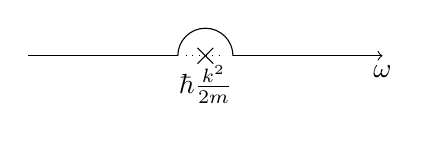
\begin{tikzpicture}
\draw (-2.25,0) -- (-0.35,0);
\draw [->] (0.35,0) -- (2.25,0) node [below]{$\omega$};
\draw (0,0) node [below]{$\hbar\frac{\mt{k}^2}{2\mt{m}}$};
\draw [dotted] (-0.25,0) --(0.25,0);
\draw (-0.1,-0.1) -- (0.1,0.1);
\draw (-0.1,0.1) -- (0.1,-0.1);
\draw (-0.35,0)  arc (180:0:0.35);
\end{tikzpicture}

fig. b
\end{center}
\end{minipage}
\vspace{0.3cm}

% 68
On peut encore dire que sans déplacer le pôle, on l'a contourmné par
un demi-cercle de rayon infiniment petit $\epsilon$ dans le demi-plan supérieur
(fig. b) (c'est en effet ainsi que l'on interprète l'intégration si on
remplace dans (14) non pas la forme (20) mais la forme (18) de G$_{(+)}$)

De même pour G$_-$, on a les deux intégrations équivalentes schématisées par les fig. a' et b' :

\vspace{0.3cm}
\begin{minipage}[c]{.45\linewidth}
\begin{center} \begin{tikzpicture}
\draw [->] (-2.25,0) -- (2.25,0) node [below]{$\omega$};
\draw (0,0.07) -- (0,-0.07) node [below]{$\hbar\frac{\mt{k}^2}{2\mt{m}}$};
\draw [dotted] (0,0) --(0,0.7);
\draw (0,0.6) node [below right]{$\epsilon$};
%\draw (2.95,-0.7) ;
\draw (-0.1,0.8) -- (0.1,0.6);
\draw (-0.1,0.6) -- (0.1,0.8);
\end{tikzpicture}

fig. a'
\end{center}
\end{minipage}
\hfill
\begin{minipage}[c]{.45\linewidth}
\begin{center} \begin{tikzpicture}
\draw (-2.25,0) -- (-0.35,0);
\draw [->] (0.35,0) -- (2.25,0) node [below]{$\omega$};
\draw (0,0) node [above right]{$\hbar\frac{\mt{k}^2}{2\mt{m}}$};
\draw [dotted] (-0.25,0) --(0.25,0);
\draw (-0.1,-0.1) -- (0.1,0.1);
\draw (-0.1,0.1) -- (0.1,-0.1);
\draw (-0.35,0)  arc (-180:0:0.35);
\end{tikzpicture}

fig. b'
\end{center}
\end{minipage}
\vspace{0.3cm}

Pour calculer l'intégrale en $\omega$ de (22), nous allons utiliser la méthode
des résidus qui consiste à fermer le contour d'intégration de l'axe réel
par un demi-cercle de rayon tendant vers l'infini et sur lequel l'intégrale
à calculer tend vers zéro. Deux cas se présentent alors :

$\alpha$) t$_2-$t$_1<0$: Pour que $|\mt{e}^{-\mt{i}\omega(\mt{t}_2-\mt{t}_1)}|$ tende vers zéro, sur le grand
cercle, la partie imaginaire de $\omega$ doit être positive et le demi-grand
cercle doit se trouver dans le demi-plan supérieur. Alors G$_+$ n'a pas de
pôles à l'intérieur du contour d'intégration et la méthode des résidus
nous donne K$_{(+)}=0$.

$\beta$) t$_2-$t$_1>0$: il faut au contraire fermer le contour par un demi-cercle
dans le demi-plan inférieur et on a alors K$_{(-)}=0$.

% 69
Nous avons ainsi établi les relations annoncées (21-a) et (21-b) et
K$_+$ est bien la fonction de Green retardée de la particule libre. Nous
allons maintenant achever de la calculer.

\ul{Calcul de K$_+$(2,1)} :

Pour t$_2$ > t$_1$ nous avons vu qu'il faut fermer le contour
d'intégration par un demi-grand cercle dans le demi-plan inférieur.
Il est facile de s'assurer que l'intégrale sur ce demi-grand cercle
tend vers zéro et on a :
\[
\lim_{\epsilon\to\,0_\pm}\int\frac{\mt{d}\omega\mt{ e}^{-\mt{i}\omega(\mt{t}_2-\mt{t}_1)}}{\hbar\omega-\frac{\hbar^2\mt{k}^2}{2\mt{m}}+\mt{i}\epsilon}=
-2\mt{i}\pi\lim_{\epsilon\to\,0_+}\mt{Résidu}\left[\frac{\mt{ e}^{-\mt{i}\omega(\mt{t}_2-\mt{t}_1)}}{\hbar\omega-\frac{\hbar^2\mt{k}^2}{2\mt{m}}+\mt{i}\epsilon}\right]=
-\frac{2\mt{i}\pi}{\hbar}\mt{ e}^{-\mt{i}\frac{\hbar\mt{k}^2}{2\mt{m}}(\mt{t}_2-\mt{t}_1)}
\]

La relation (22) devient alors :
\[
\tag{23}\mt{K}_+(2,1)=\frac{1}{(2\pi)^3}
\iiint\mt{d}^3\mt{k}\mt{ e}^{\mt{i}\vec{\mt{k}}(\vec{\mt{r}}_2-\vec{\mt{r}}_1)}
\mt{ e}^{-\mt{i}\frac{\hbar\mt{k}^2}{2\mt{m}}(\mt{t}_2-\mt{t}_1)}
\]
\[
=\left[\frac{1}{2\pi}
\int\mt{d}\mt{k}_\mt{x}\mt{ e}^{\mt{i}\mt{k}_x(\mt{x}_2-\mt{x}_1)}
\mt{ e}^{-\mt{i}\frac{\hbar\mt{k}_\mt{x}^2}{2\mt{m}}(\mt{t}_2-\mt{t}_1)}\right]\times
\mt{(intégrales analogues en y et z)}
\]


Faisons le changement de variable p $=\hbar$k$_\mt{x}$ , L'intégration sur k devient
\[
\frac{1}{2\pi\hbar}
\int\mt{d}\mt{p}\mt{ e}^{\frac{\mt{i}}{\hbar}\left[\mt{p}(\mt{x}_2-\mt{x}_1)
-\frac{\mt{p}^2}{2\mt{m}}(\mt{t}_2-\mt{t}_1)\right]}
\]

intégrale que nous avons déjà calculée au chapitre II, \S 2  et qui
représente précisément le propagateur $<$ x$_2$t$_2\,|\,$x$_1$t$_1>$ à une dimension
(formule (7) du chapitre II).

% 70
On trouve finalement, en tenant compte de la condition K$_{(+)}=0$ si t$_2<$ t$_1$

\[
\tag{24}\mt{K}_{(+)}(\vec{\mt{r}}_2-\vec{\mt{r}}_1,\mt{t}_2-\mt{t}_1)=
\theta(\mt{t}_2-\mt{t}_1)\mt{e}^{-\frac{3\mt{i}\pi}{4}}
\left[\frac{\mt{m}}{2\pi\hbar(\mt{t}_2-\mt{t}_1)}\right]^\frac{3}{2}
\mt{ exp }\frac{\mt{im}}{2\hbar}\frac{(\vec{\mt{r}}_2-\vec{\mt{r}}_1)}{\mt{t}_2-\mt{t}_1}
\]
Le formule (24) n'est autre que l'extension au problème à trois dimensions
de la formule (7) du chapitre II.

\subsection{Equation des potentiels}% 2°) 

L'équation satisfaite en électromagnétisme par le potentiel
scalaire V est
\[
(\Delta-\frac{1}{\mt{c}^2}\frac{\partial^2}{\partial\mt{t}^2})\mt{K}_+(2,1)=-\frac{\rho}{\epsilon_0}
\]
Cherchons la fonction de Green retardée de cette équation, c'est-à-dire
la distribution K, (2, 1) vérifiant les relations :
\[
\tag{25-a}\left[\Delta_2-\frac{1}{\mt{c}^2}\frac{\partial^2}{\partial\mt{t}_2^2}\right]\mt{K}_+(2,1)=
\delta(\vec{\mt{r}}_2-\vec{\mt{r}}_1)\ \delta(\mt{t}_2-\mt{t}_1)
\]
\[
\tag{25-b}\mt{K}_+(2,1)=0\ \ \ \ \ \mt{si}\ \ \ \ \ \mt{t}_2<\mt{t}_1
\]
Il est évident, en raison de l'invariance du problème par translation, que
K$_+$(2,1) n'est une fonction que de $\vec{\mt{r}}_2-\vec{\mt{r}}_1$ et $\mt{t}_2-\mt{t}_1$. Faisons, comme pour
la fonction de Creen de la particule libre, l'hypothèse que K$_+$(2,1) a une
transformée de Fourier G$_+(\vec{\mt{k}},\omega)$ définie par la relation
\[
\tag{26}\mt{K}_+(2,1)=\frac{1}{(2\pi)^4}\int\!\!...\!\!\int \mt{G}_+(\vec{\mt{k}},\omega)
\ \mt{e}^{\mt{i}\left[\vec{\mt{k}}(\vec{\mt{r}}_2-\vec{\mt{r}}_1)-\omega(\mt{t}_2-\mt{t}_1)\right]}
\mt{d}^3\vec{\mt{k}}\ \mt{d}\omega
\]
La transformée de Fourier de (25-a) nous conduit à : 
\[
\tag{27}\left[-\mt{k}^2+\frac{1}{c^2}\omega^2\right]\mt{G}_+(\vec{\mt{k}},\omega)=1
\]
 
% 71
Nous avons ainsi, comme pour la particule libre, remplacé
l'équation aux dérivées partielles (25-a) par une équation algébrique
dont l'inconnue est la distribution G$_+(\vec{\mt{k}},\omega)$. Le problème est cependant
plus compliqué, car la quantité $\frac{\omega^2}{\mt{c}^2}-\mt{k}^2$ possède deux zéros $\omega=\pm$ck

Il est très facile de vérifier qu'une solution particulière
de (27-a) est
\[
\mt{G}_+(\vec{\mt{k}},\omega)=
\frac{\mt{c}}{2\mt{k}}\left\{\mc{P}\left[\frac{1}{\omega-\mt{ck}}\right]-\mc{P}\left[\frac{1}{\omega+\mt{ck}}\right]\right\}
\]

A cette solution particulière, il faut ajouter la solution générale de
l'équation homogène $[\frac{\omega^2}{\mt{c}^2}-\mt{k}^2]$G$\vec{\mt{k},\omega}=0$, qui est $-\frac{\mt{c}}{2\mt{k}}[\lambda\delta(\omega-\mt{ck})-\lambda'\delta(\omega+\mt{ck})]$ ($\lambda$ et $\lambda'$
 nombres complexes quelconques)

Finalement, la solution générale de (27) est
\[
\mt{G}_+(\vec{\mt{k}},\omega)=
\frac{\mt{c}}{2\mt{k}}\left\{\mc{P}\left[\frac{1}{\omega-\mt{ck}}\right]-\lambda\delta(\omega-\mt{ck})-\mc{P}\left[\frac{1}{\omega+\mt{ck}}\right]+\lambda'\delta(\omega+\mt{ck})\right\}
\]

Elle dépend des deux constantes complexes $\lambda$ et $\lambda'$. Comme pour la particule
libre, envisageons a priori les quatre solutions correspondant à
\begin{center}
$\begin{array}{r c l}
\lambda & = & \alpha\mt{i}\pi \ \ \ \ \ (\mt{ avec }\alpha\mt{ et }\alpha'=\pm1)\\
\lambda' & = & \alpha'\mt{i}\pi
\end{array}$
\end{center}
Elles peuvent s'écrire
\[
\mt{G}_+(\vec{\mt{k}},\omega)=\lim_{\epsilon\to\,0_+}
\frac{\mt{c}}{2\mt{k}}\left[\frac{1}{\omega-\mt{ck}+\alpha\mt{i}\epsilon}-\frac{1}{\omega+\mt{ck}+\alpha'\mt{i}\epsilon}\right]
\]

Nous avons ainsi obtenu quatre distributions G$(\vec{\mt{k}},\omega)$ pour lesquelles les
pôles $\omega=\pm\mt{ck}$ sont déplacés d'une quantité infiniment petite dans le
plan complexe au-dessus ou au-dessous de l'axe réel, On peut encore dire
que dans les intégrations où intervient G$(\vec{\mt{k}},\omega)$, il existe quatre facons
de contourner par un demi-cercle de rayon infiniment petit $\epsilon$ les pôles $\omega=\pm\mt{ck}$

% 72
De façon précise,
\ul{à $\alpha=\alpha'=+1$}, il correspond %%%%%%%%%%%%%%%%%%%%%%%  1

\vspace{0.3cm}
\begin{minipage}[c]{.45\linewidth} \begin{center}
la configuration

\begin{tikzpicture}
\draw [->] (-2.25,0) -- (2.25,0) node [below]{$\omega$};
\draw (-0.95,-0.07) -- (-0.95,0.07) node [above]{-ck};
\draw [dotted] (-0.95,0) -- (-0.95,-0.7); \draw (-1.05,-0.8) -- (-0.85,-0.6); \draw (-1.05,-0.6) -- (-0.85,-0.8);
\draw (0.95,-0.07) -- (0.95,0.07) node [above]{+ck};
\draw [dotted] (0.95,0) -- (0.95,-0.7); \draw (0.85,-0.8) -- (1.05,-0.6); \draw (0.85,-0.6) -- (1.05,-0.8);
\end{tikzpicture} \end{center} \end{minipage}
\hfill
\begin{minipage}[c]{.45\linewidth} \begin{center}
ou le contour d'intégration \vspace{0.3cm}

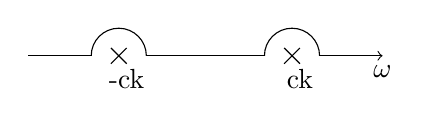
\begin{tikzpicture}
\draw (-2.25,0) -- (-1.45,0); \draw (-0.75,0) -- (0.75,0); \draw [->] (1.45,0) -- (2.25,0) node [below]{$\omega$};
\draw (-1,-0.05) node [below]{-ck}; \draw (1.2,-0.05) node [below]{ck};
\draw (-1.2,-0.1) -- (-1,0.1); \draw (-1.2,0.1) -- (-1,-0.1); \draw (-1.45,0)  arc (180:0:0.35);
\draw (1,-0.1) -- (1.2,0.1); \draw (1,0.1) -- (1.2,-0.1); \draw (0.75,0)  arc (180:0:0.35);
\end{tikzpicture} \end{center} \end{minipage}
\vspace{0.3cm}

\ul{à $\alpha=\alpha'=-1$} %%%%%%%%%%%%%%%%%%%%%%%%  2

\vspace{0.3cm}
\begin{minipage}[c]{.45\linewidth} \begin{center}
\begin{tikzpicture}
\draw [->] (-2.25,0) -- (2.25,0) node [below]{$\omega$};
\draw (-0.95,-0.07) -- (-0.95,0.07) node [below]{-ck};
\draw [dotted] (-0.95,0) -- (-0.95,0.7); \draw (-1.05,0.8) -- (-0.85,0.6); \draw (-1.05,0.6) -- (-0.85,0.8);
\draw (0.95,-0.07) -- (0.95,0.07) node [below]{+ck};
\draw [dotted] (0.95,0) -- (0.95,0.7); \draw (0.85,0.8) -- (1.05,0.6); \draw (0.85,0.6) -- (1.05,0.8);
\end{tikzpicture} \end{center} \end{minipage}
\hfill
\begin{minipage}[c]{.45\linewidth} \begin{center}
\vspace{0.3cm}
ou \hspace {0.3cm}
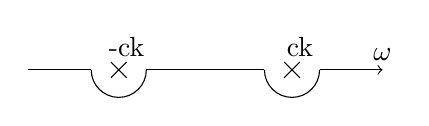
\begin{tikzpicture}
\draw (-2.25,0) -- (-1.45,0); \draw (-0.75,0) -- (0.75,0); \draw [->] (1.45,0) -- (2.25,0) node [above]{$\omega$};
\draw (-1,0.05) node [above]{-ck}; \draw (1.2,0.05) node [above]{ck};
\draw (-1.2,-0.1) -- (-1,0.1); \draw (-1.2,0.1) -- (-1,-0.1); \draw (-1.45,0)  arc (-180:0:0.35);
\draw (1,-0.1) -- (1.2,0.1); \draw (1,0.1) -- (1.2,-0.1); \draw (0.75,0)  arc (-180:0:0.35);
\end{tikzpicture} \end{center} \end{minipage}
\vspace{0.3cm}

\ul{à $\alpha=1;\ \alpha'=-1$} %%%%%%%%%%%%%%%%%%%%%%%%  3

\vspace{0.3cm}
\begin{minipage}[c]{.45\linewidth} \begin{center}
\begin{tikzpicture}
\draw [->] (-2.25,0) -- (2.25,0) node [below]{$\omega$};
\draw (-0.95,-0.07) -- (-0.95,0.07) node [below]{-ck};
\draw [dotted] (-0.95,0) -- (-0.95,0.7); \draw (-1.05,0.8) -- (-0.85,0.6); \draw (-1.05,0.6) -- (-0.85,0.8);
\draw (0.95,-0.07) -- (0.95,0.07) node [above]{+ck};
\draw [dotted] (0.95,0) -- (0.95,-0.7); \draw (0.85,-0.8) -- (1.05,-0.6); \draw (0.85,-0.6) -- (1.05,-0.8);
\end{tikzpicture} \end{center} \end{minipage}
\hfill
\begin{minipage}[c]{.45\linewidth} \begin{center}
\vspace{0.3cm}
ou \hspace {0.3cm}
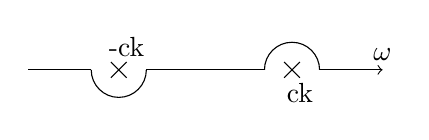
\begin{tikzpicture}
\draw (-2.25,0) -- (-1.45,0); \draw (-0.75,0) -- (0.75,0); \draw [->] (1.45,0) -- (2.25,0) node [above]{$\omega$};
\draw (-1,0.05) node [above]{-ck}; \draw (1.2,-0.05) node [below]{ck};
\draw (-1.2,-0.1) -- (-1,0.1); \draw (-1.2,0.1) -- (-1,-0.1); \draw (-1.45,0)  arc (-180:0:0.35);
\draw (1,-0.1) -- (1.2,0.1); \draw (1,0.1) -- (1.2,-0.1); \draw (0.75,0)  arc (180:0:0.35);
\end{tikzpicture} \end{center} \end{minipage}
\vspace{0.3cm}

\ul{à $\alpha=-1;\ \alpha'=1$} %%%%%%%%%%%%%%%%%%%%%%%%  4

\vspace{0.3cm}
\begin{minipage}[c]{.45\linewidth} \begin{center}
\begin{tikzpicture}
\draw [->] (-2.25,0) -- (2.25,0) node [below]{$\omega$};
\draw (-0.95,-0.07) -- (-0.95,0.07) node [above]{-ck};
\draw [dotted] (-0.95,0) -- (-0.95,-0.7); \draw (-1.05,-0.8) -- (-0.85,-0.6); \draw (-1.05,-0.6) -- (-0.85,-0.8);
\draw (0.95,-0.07) -- (0.95,0.07) node [below]{+ck};
\draw [dotted] (0.95,0) -- (0.95,0.7); \draw (0.85,0.8) -- (1.05,0.6); \draw (0.85,0.6) -- (1.05,0.8);
\end{tikzpicture} \end{center} \end{minipage}
\hfill
\begin{minipage}[c]{.45\linewidth} \begin{center}
\vspace{0.3cm}
ou \hspace {0.3cm}
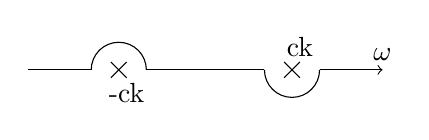
\begin{tikzpicture}
\draw (-2.25,0) -- (-1.45,0); \draw (-0.75,0) -- (0.75,0); \draw [->] (1.45,0) -- (2.25,0) node [above]{$\omega$};
\draw (-1,-0.05) node [below]{-ck}; \draw (1.2,0.05) node [above]{ck};
\draw (-1.2,-0.1) -- (-1,0.1); \draw (-1.2,0.1) -- (-1,-0.1); \draw (-1.45,0)  arc (180:0:0.35);
\draw (1,-0.1) -- (1.2,0.1); \draw (1,0.1) -- (1.2,-0.1); \draw (0.75,0)  arc (-180:0:0.35);
\end{tikzpicture} \end{center} \end{minipage}
\vspace{0.3cm}

Chacune de ces quatre distributions G$(\vec{\mt{k}},\omega)$ correspond à une fonction
K(2,1) vérifiant des conditions aux limites particulières.

Pour calculer l'intégrale en $\omega$ de (26) par la méthode des résidus, dans
le cas où t$_2-$t$_1<$ 0, il faut fermer le contour d'intégration par un
demi-cercle dans le demi-plan supérieur et c'est donc la première configuration $\alpha=\alpha'=+1$ qui convient pour donner un résultat nul.

La transformée de la fonction de Green cherchée est donc
\[
\mt{G}_+(\vec{\mt{k}},\omega)=\lim_{\epsilon\to\,0_+}
\frac{\mt{c}}{2\mt{k}}\left\{\frac{1}{\omega+\mt{i}\epsilon-\mt{ck}}-\frac{1}{\omega+\mt{i}\epsilon+\mt{ck}}\right\}
\]
\[
\tag{28}\mt{G}_+(\vec{\mt{k}},\omega)=\lim_{\epsilon\to\,0_+}\frac{1}{\frac{(\omega+\mt{i}\epsilon)^2}{\mt{c}^2}-\mt{k}^2}
\]

% 73
L'intégration (26) nous conduit alors à la fonction de Green
retardée K(2,1). On intègre sur $\omega$ par la méthode des résidus :
\[
\lim_{\epsilon\to\,0_+}\int_{-\infty}^{\infty}\frac{\mt{e}^{-\mt{i}\omega(\mt{t}_2-\mt{t}_1)}}{\frac{(\omega+\mt{i}\epsilon)^2}{\mt{c}^2}-\mt{k}^2}\mt{d}\omega=
-2\mt{i}\pi\ \theta(\mt{t}_2-\mt{t}_1)\lim_{\epsilon\to\,0_+}\sum\mt{Résidu}\left[\frac{\mt{e}^{-\mt{i}\omega(\mt{t}_2-\mt{t}_1)}}{\frac{(\omega+\mt{i}\epsilon)^2}{\mt{c}^2}-\mt{k}^2}\right]
\]
\[
=2\mt{i}\pi\mt{ c }\theta(\mt{t}_2-\mt{t}_1)\left[\frac{\mt{e}^{\mt{ikc}(\mt{t}_2-\mt{t}_1)}-\mt{e}^{-\mt{ikc}(\mt{t}_2-\mt{t}_1)}}{2\mt{k}}\right]
\]
(26) donne alors :
\[
\mt{K}_+(2,1)=\frac{\mt{ic}}{(2\pi)^3}\iiint \mt{e}^{\mt{i}\vec{\mt{k}}(\vec{\mt{r}}_2-\vec{\mt{r}}_1)}\frac{\mt{e}^{\mt{ikc}(\mt{t}_2-\mt{t}_1)}-\mt{e}^{-\mt{ikc}(\mt{t}_2-\mt{t}_1)}}{2\mt{k}}\theta(\mt{t}_2-\mt{t}_1)\vec{\mt{d}^3\mt{k}}
\]

En passant en coordonnées sphériques, l'axe Oz étant dirigé suivant $\vec{\mt{r}}_2-\vec{\mt{r}}_1$, $\int\vec{\mt{d}^3\mt{k}}$
 devient $\int2\pi\mt{k}^2\mt{ dk}\mt{ sin }\psi\mt{ d}\psi$ et
\[
\mt{K}_+(2,1)=\frac{\mt{ic }\theta(\mt{t}_2-\mt{t}_1)}{(2\pi)^2}\int_0^\pi\int_0^\infty \mt{e}^{\mt{ik}|\vec{\mt{r}}_2-\vec{\mt{r}}_1|\mt{cos}\psi}\left(\frac{\mt{e}^{\mt{ikc}(\mt{t}_2-\mt{t}_1)}-\mt{e}^{-\mt{ikc}(\mt{t}_2-\mt{t}_1)}}{2}\right)\mt{k sin}\psi\mt{ dk d}\psi
\]
Posons t$_2-$t$_1=\tau$, $|\vec{\mt{r}}_2-\vec{\mt{r}}_1|=\,$r et effectuons l'intégration sur $\psi$ : il
vient :
\[
\mt{K}_+(2,1)=\frac{1}{(2\pi)^2}\ \frac{\mt{c}}{2\mt{r}}\ \theta(\tau) \int_0^\infty (\mt{e}^{\mt{ikr}}-\mt{e}^{-\mt{ikr}}) (\mt{e}^{\mt{ikc}\tau}-\mt{e}^{-\mt{ikc}\tau})\mt{ dk}
\]
Soit
\[
\mt{K}_+(2,1)=\frac{1}{(2\pi)^2}\ \frac{\mt{c}}{2\mt{r}}\ \theta(\tau) \int_0^\infty \left[\mt{e}^{\mt{ik(r+c}\tau)}+\mt{e}^{-\mt{ik(r+c}\tau)}-\mt{e}^{\mt{ik(r-c}\tau)}-\mt{e}^{-\mt{ik(r-c}\tau)}\right]\mt{ dk}
\]
\[
=\frac{1}{(2\pi)^2}\ \frac{\mt{c}}{2\mt{r}}\ \theta(\tau) \int_{-\infty}^\infty \left[\mt{e}^{\mt{ik(r+c}\tau)}-\mt{e}^{\mt{ik(r-c}\tau)}\right]\mt{ dk}
\]
\[
=\frac{\mt{c}}{4\pi\mt{r}}\ \theta(\tau) \big[\delta(\mt{r+c}\tau)-\delta(\mt{r-c}\tau)\big]
\]

% 74
r $=|\vec{\mt{r}}_2-\vec{\mt{r}}_1|$ est positif. Le terme $\theta(\tau)$ permet donc de supprimer la
distribution $\delta$(r + c$\tau$) et finalement :
\[
\tag{29}\mt{K}_+(2,1)=-\frac{\mt{1}}{4\pi\mt{r}}\ \delta(\mt{r-c}\tau)\ \theta(\tau)=-\frac{\mt{c}}{4\pi\mt{r}}\ \delta(\tau-\frac{\mt{r}}{\mt{c}})\ \theta(\tau)
\]

\[
=-\frac{1}{4\pi|\vec{\mt{r}}_2-\vec{\mt{r}}_1|}\ \delta\left[\mt{t}_2-\mt{t}_1-\frac{|\vec{\mt{r}}_2-\vec{\mt{r}}_1|}{\mt{c}}\right]\ \theta(\mt{t}_2-\mt{t}_1)
\]
On en déduit immédiatement le potentiel au point $\vec{\mt{r}}_2$, t$_2$  en présence d'une
distribution de charges $\rho(\vec{\mt{r}}_1$, t$_1)$ :
\[
\tag{30}\mt{V}(\vec{\mt{r}}_2, t_2)=\frac{1}{4\pi\epsilon_0}\ \int \rho(\vec{\mt{r}}_1, \mt{t}_1)\ \frac{1}{|\vec{\mt{r}}_2-\vec{\mt{r}}_1|}\ 
\delta\left[\mt{t}_2-\mt{t}_1-\frac{|\vec{\mt{r}}_2-\vec{\mt{r}}_1|}{\mt{c}}\right]\mt{d}^3\vec{\mt{r}_1}\mt{ dt}_1
\]
\[
=\frac{1}{4\pi\epsilon_0}\ \int \frac{\rho(\vec{\mt{r}}_1, \mt{t}_2-\frac{|\vec{\mt{r}}_2-\vec{\mt{r}}_1|}{\mt{c}})}{|\vec{\mt{r}}_2-\vec{\mt{r}}_1|}
\mt{d}^3\vec{\mt{r}_1}
\]
(30) n'est autre que l'équation bien connue des "potentiels retardés" que
l'on retrouve ainsi à partir de la fonction de Green du d'Alembertien.

\ul{Remarque} : La condition aux limites imposée à la fonction de Green K$_+$(2,1)
fait jouer au temps un rôle privilégié. Dans la transformée de Fourier
G$_+(\vec{\mt{k}}, \omega)$, c'est $\omega$ qui est particularisé (cf relation (28) ). On voit ainsi
que cette condition ne satisfait pas à l'invariance relativiste. Nous verrons qu'en relativité, il faut imposer à la fonction de Green d'autres conditions, satisfaisant à l'invariance relativiste et qui correspondent à des
contours d'intégration pour lesquels les pôles $\pm$ck sont repoussés de part
et d'autre de l'axe réel.
% 75

\ul{En conclusion} : Nous avons montré que la technique de la transformation
de Fourier nous permet de calculer les fonctions de Green des équations
aux dérivées partielles à coefficients constants. Les conditions aux
limites se traduisent simploment par un déplacement dans le plan complexe,
dans un sens bien déterminé, des pôles de cette transformée de Fourier,
Cette propriété nous permet de tenir compte de \ul{façon analytiquement} simple
du \ul{principe physique de causalité} (K = O si t < t).

Nous allons maintenent appliquer les techniques des fonctions
de Green à la théorie des perturbations :

\section{Développement en série de perturbations}% E.

Soit un système quantique dont l'évolution est décrite par un
hamiltonien H$_0$. Supposons connue sa fonction de Green retardée K$_0$(2,1).
Elle vérifie les relations :
\[
\tag{31-a}\left[\mt{i}\hbar\frac{\partial}{\partial \mt{t}_2}-\mt{H}_0(2)\right]\mt{K}_0(2,1)=\mt{i}\hbar\delta_4(2,1)
\]
\[
\tag{31-b}\mt{K}_{0+}(2,1)=0\ \ \ \ \ \mt{si} \ \ \ \ \ \mt{t}_2<\mt{t}_1
\]
Appliquons maintenant une perturbation V (dépendante au indépendante du
temps). Le hamiltonien devient H = H$_0$ + V. Cherchons à déterminer, à partir
de K$_{0+}$ et de V, la fonction de Green retardée du hamiltonien H, c'est-à-dire
la distribution K$_+$(2,1) vérifiant :
\[
\tag{32-a}\left[\mt{i}\hbar\frac{\partial}{\partial \mt{t}_2}-\mt{H}(2)\right]\mt{K}(2,1)=\mt{i}\hbar\delta_4(2,1)
\]
\[
\tag{32-b}\mt{K}_+(2,1)=0\ \ \ \ \ \mt{si} \ \ \ \ \ \mt{t}_2<\mt{t}_1
\]
Pour cela, écrivons l'équation (32-a) sous la forme inhomogène :
\[
\left[\mt{i}\hbar\frac{\partial}{\partial \mt{t}_2}-\mt{H}_0(2)\right]\mt{K}_+(2,1)=\mt{i}\hbar\delta_4(2,1)+\mt{V}(2)\mt{K}(2,1)
\]
et considérons formellement le second membre comme une source $\rho$(2).

% 76

Nous avons vu alors (\S 3) que si K'(2,1) vérifie
\[
\tag{33}\left[\mt{i}\hbar\frac{\partial}{\partial \mt{t}_2}-\mt{H}_0(2)\right]\mt{K'}(2,1)=\delta_4(2,1)
\]
alors
\[
\tag{34}\mt{K}_+(2,1)=\int\rho(3)\mt{ K'}(2,3)\mt{ d}3
\]
Or, d'après (31-a), on voit que K'(2, 1) = $\frac{\mt{K}_{0+}(2,1)}{\mt{i}\hbar}$.
(34) s'écrit alors
\[
\mt{K}_+(2,1)=\frac{1}{\mt{i}\hbar}\int\mt{K}_{0+}(2,3)\big[\mt{i}\hbar\ \delta_4(3,1)+\mt{V}(3)\mt{ K}_+(3,1)\big]\mt{ d}3
\]
Soit :
\[
\tag{35}\mt{K}_+(2,1)=\mt{K}_{0+}(2,1)+\frac{1}{\mt{i}\hbar}\int\mt{K}_{0+}(2,3)\mt{ V}(3)\mt{ K}_+(3,1)\mt{ d}3
\]

Il est facile de montrer que K$_+$(2,1), défini par l'équation (35),
satisfait bien à l'équation (32-a). Nous montrons dans la suite qu'elle
satisfait à la relation (32-b). les deux fonctions de Green retardées
du hamiltonien non perturbé et du hamiltonien perturbé sont donc reliées
entre elles par \ul{l'équation intégrale (35)}.

Nous pouvons, dans le second membre de (35), remplacer K$_+$(3, 1)
par son expression intégrale et on obtient ainsi par itération le \ul{développement
en série de Neumann-Liouville} de la perturbation :
\[
\tag{36}\mt{K}_+(2,1)=\mt{K}_{0+}(2,1)+\frac{1}{\mt{i}\hbar}\int\mt{K}_{0+}(2,3)\mt{ V}(3)\mt{ K}_{0+}(3,1)\mt{ d}3
\]
\[
+(\frac{1}{\mt{i}\hbar})^2\int\mt{K}_{0+}(2,3)\mt{ V}(3)\mt{ K}_{0+}(3,4)\mt{ V}(4)\mt{ K}_{0+}(4,1)\mt{ d}3\mt{ d}4 + ...
\]

Dans chaque terme de la série (36), la présence des fonctions de
Green retardées K$-{0+}$ fait que les temps sont automatiquement rangés par
ordre croissant entre t$_1$ et t$_2$ : par exenple, le troisième terme est nul
% 77
à moins que l'on ait simultanément  t$_2\geqslant$ t$_3$; t$_3\geqslant$ t$_4$; t$_4\geqslant$ t$_1$. Il est donc
nul si t$_2<$ t$_1$. Il en est de même de tous les termes de ce développement.
La solution de l'équation (35) est donc bien telle que K$_+$(2, 1) = 0 si
t$_2<$ t$_1$. C'est donc bien la \ul{fonction de Green retardée} du système perturbé.

\ul{Remarques} :
Dans le développement (36), les intégrations sur les variables 3, 4, etc.
(c'est-à-dire sur $\vec{\mt{r}}_3$,$\mt{t}_3$; $\vec{\mt{r}}_4$,$\mt{t}_4$, etc.) sont libres et s'étendent à l'espace-temps tout entier.
Les conditions aux limites sur les fonctions de Green
sont \ul{implicitement} contenues dans les intégrales et annulent toutes les contributions
autres que t$_2\geqslant$ ... $\geqslant$ t$_3\geqslant$ t$_1$. Le développement (36) correspond
à une simplification notable de l'écriture par rapport au développerent
classique de le page 41 (formule (27) ). Cette simplification est \ul{effective}
car nous avons vu qu'on peut tenir compte des conditions aux limites de façon
mathématiquement simple.
\section{Représentation diagrammatique du développement de Neumann-Liouville}% F.

Nous allons définir une convention qui va nous permettre d'associer un diagramme à chaque terme du développement (36).

\ul{Conventions} :

a) Les temps sont représentés en ordonnée, croissant de bas en
haut, et en abscisse, on portera une "variable d'espace".

b) A chaque terme K$_{0+}$(i, j) sera associée une ligne \ul{pointillée}
joignant i et j

\vspace{0.3cm}
\begin{minipage}[c]{.45\linewidth} \begin{center}
\begin{tikzpicture}
\draw [dashed] (0,-1) node [left]{j} -- (0,1) node [left]{i};
\draw (-0.1,-1.1) -- (0.1,-0.9); \draw (-0.1,-0.9) -- (0.1,-1.1);
\draw (-0.1,1.1) -- (0.1,0.9); \draw (-0.1,0.9) -- (0.1,1.1);
\draw (-0.2,-0.1) -- (0,0.1); \draw (0,0.1) -- (0.2,-0.1) node [right]{\ \ \ K$_{0+}$(i, j)};
\end{tikzpicture} \end{center} \end{minipage}
\hfill
\begin{minipage}[c]{.45\linewidth} \begin{center}
\begin{tikzpicture}
\draw (0,-1) node [left]{j} -- (0,1) node [left]{i};
\draw (-0.1,-1.1) -- (0.1,-0.9); \draw (-0.1,-0.9) -- (0.1,-1.1);
\draw (-0.1,1.1) -- (0.1,0.9); \draw (-0.1,0.9) -- (0.1,1.1);
\draw (-0.2,-0.1) -- (0,0.1); \draw (0,0.1) -- (0.2,-0.1) node [right]{\ \ \ K$_+$(i, j)};
\end{tikzpicture} \end{center} \end{minipage}
\vspace{0.3cm}

c) A chaque terme K$_+$(i, j) sera associée une ligne \ul{pleine} joignant i et j.

d) A chaque terme V (i) un cercle autour du point i.

% 78
On associe ainsi à chaque intégrale du déveloprement (36) un
diagramme, Chaque diagramme est affecté d'un facteur de poids $(\frac{1}{\mt{i}\hbar})^n$, où n
représente le nombre de cercles du diagramme, et pour obtenir le terme du
développement (36) associé, il faut intégrer librement sur les variables
entourées d'un cercle. On obtient alors le développement diagrammatique :
\begin{flushright}
\begin{tikzpicture}
\def\espace{2.3}
\draw (-0.25,-1.5) node {$\bullet$} node [left]{1} -- (0.25,1.5) node {$\bullet$} node [left]{2};
\draw (\espace/2,0) node{\bf{=}};

\draw [dashed] (\espace-0.25,-1.5) node {$\bullet$} node [left]{1} -- (\espace+0.25,1.5) node {$\bullet$} node [left]{2};
\draw (3*\espace/2,0) node{\bf{+}};

\draw [dashed] (2*\espace-0.25,-1.5) node {$\bullet$} node [left]{1} -- (2*\espace+0.9,0) node {$\bullet$} ;
\draw (2*\espace+0.9,0) circle (0.25);
\draw (2*\espace+1.2,0.4) node {3};
\draw [dashed] (2*\espace+0.9,0) -- (2*\espace+0.25,1.5) node {$\bullet$} node [left]{2};

\draw (6.5*\espace/2,0) node{\bf{+}};

\draw [dashed] (4*\espace-0.5,-1.5) node {$\bullet$} node [left]{1} -- (4*\espace,-0.5) node {$\bullet$};
\draw (4*\espace,-0.5) circle (0.25);
\draw (4*\espace+0.4,-0.7) node {4};
\draw [dashed] (4*\espace,-0.5) -- (4*\espace+1,0.5) node {$\bullet$};
\draw (4*\espace+1,0.5) circle (0.25);
\draw (4*\espace+1.5,0.5) node {3};
\draw [dashed] (4*\espace+1,0.5) -- (4*\espace,1.5) node {$\bullet$} node [left]{2};
\draw (11*\espace/2,0) node{\bf{+ ....}};
\draw (13*\espace/2,0) node{(37)};

\end{tikzpicture} \end{flushright}

Il est évident qu'avec nos conventions, il y a correspondance
biunivoque entre chaque terme du développement diagrammatique et chaque
terme de la série (36).

Les diagrammes conduisent à une représentation physique simple de
la perturbation : \ul{l'amplitude de probabilité} pour que la particule en $\vec{\mt{r}}_1$
à l'instant t$_1$ se trouve en $\vec{\mt{r}}_2$ à l'instant t$_2$, en présence du potentiel
perturbateur V, est la somme de plusieurs contributions :

— une correspondant aux chemins où elle ne subit aucune interaction avec V

— une correspondant aux chemins où elle subit une interaction avec V

— une correspondent aux chemins où elle subit deux interactions avec V

etc...

% 79
Prenons pour exemple le \ul{diagramme de diffusion double} :
\begin{center}
\begin{tikzpicture}
\draw [dashed] (0.5,-1.5) node {$\bullet$} node [left]{1} -- (0,-0.5) node {$\bullet$};
\draw (0,-0.5) circle (0.25);
\draw (0.4,-0.7) node {4};
\draw [dashed] (0,-0.5) -- (1,0.5) node {$\bullet$};
\draw (1,0.5) circle (0.25);
\draw (1.5,0.5) node {3};
\draw [dashed] (1,0.5) -- (-1,2.5) node {$\bullet$} node [left]{2};
\end{tikzpicture} \end{center}
Ce diagramne représente une particule qui va librement (sous l'effet de
H$_0$ seul) de 1 à 4, qui est diffusée en 4 par V, qui va ensuite librement
à 3 où elle est de nouveau diffusée par V pour aller ensuite librement
jusqu'en 2. A ce chemin correspond une certaine \ul{amplitude} de probabilité.
Pour avoir la contribution des processus de diffusion double, il faut
sommer sur \ul{toutes} les positions des points intermédiaires 4 et 3. Pour
avoir la contribution de \ul{tous} les processus de diffusion, il faut ensuite
sommer tous les diarramres correspondant aux différents ordres de diffusion.
\ul{En résumé} : Pour joindre 1 à 2, plusieurs chemins sont possibles. À chaque
chemin est associée une amplitude de probabilité. Il faut sommer sur toutes
ces amplitudes pour avoir l'amplitude de probabilité globale K(2,1).
On retrouve ainsi l'idée de base de l'approche de \ul{Feynman} de la mécanique
quantique.

% 80
Remarques : $\alpha$) Les conditions aux limites sur K font que les diagrammes du type
\begin{center}
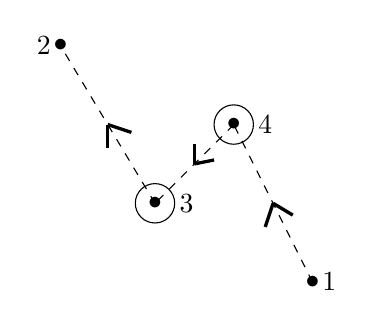
\begin{tikzpicture}
\draw [dashed] (2,-1.5) node {$\bullet$} node [right]{1} -- (1,0.5) node {$\bullet$};
\draw (1,0.5) circle (0.25);
\draw [very thick] (1.4,-0.8) -- (1.5,-0.5);\draw [very thick] (1.5,-0.5) -- (1.75,-0.65);

\draw (1.4,0.5) node {4};
\draw [dashed] (1,0.5) -- (0,-0.5) node {$\bullet$};
\draw (0,-0.5) circle (0.25);
\draw [very thick] (0.5,0.25) -- (0.5,0);\draw [very thick] (0.5,0) -- (0.75,0.05);

\draw (0.4,-0.5) node {3};
\draw [dashed] (0,-0.5) -- (-1.2,1.5) node {$\bullet$} node [left]{2};
\draw [very thick] (-0.6,0.2) -- (-0.6,0.5);\draw [very thick] (-0.6,0.5) -- (-0.3,0.4);

\end{tikzpicture} \end{center}
que nous n'avons pas exclu \ul{a priori} ont une contribution nulle.

En \ul{mécanique quantique non relativiste}, de tels diagrammes n'ont
pas de signification physique. Ils correspondent en effet à un retour du
chemin dans le passé où encore à la présence de trois particules entre les
instants t$_3$ et t$_4$.

En \ul{mécanique quantique relativiste}, ils ont au contraire une
signification, car il existe alors une possibilité de création et d'annihilation
de particules (le nombre de particules n'est plus une constante
du mouvement).

Par exemple, dans le cas où la particule est un électron, nous
verrons que le diagramme représente un électron partant de 1 à l'instant t$_1$,
voyant apparaître une paire électron-positron sous l'effet du potentiel V
à l'instant t$_3$, annihilé par le positron de la paire à l'instant t$_4$ tandis
que l'électron de la paire arrive en 2 à l'instant t$_2$. Le positron s'interprète
alors naturellement comme un électron d'énergie négative se propageant
dans le sens inverse du temps (théorie de Feynman du positron).
% 81

$\beta$) Avec les conventions adoptées, l'équation intégrale (35) peut se
représenter par le diagramme :
\begin{flushright}
\begin{tikzpicture}
\def\espace{2.3}
\draw (-0.25,-1.5) node {$\bullet$} node [left]{1} -- (0.25,1.5) node {$\bullet$} node [left]{2};
\draw (\espace/2,0) node{\bf{=}};

\draw [dashed] (\espace-0.25,-1.5) node {$\bullet$} node [left]{1} -- (\espace+0.25,1.5) node {$\bullet$} node [left]{2};
\draw (3*\espace/2,0) node{\bf{+}};

\draw (2*\espace-0.25,-1.5) node {$\bullet$} node [left]{1} -- (2*\espace+0.9,0) node {$\bullet$} ;
\draw (2*\espace+0.9,0) circle (0.25);
\draw (2*\espace+1.35,0.1) node {3};
\draw [dashed] (2*\espace+0.9,0) -- (2*\espace+0.25,1.5) node {$\bullet$} node [left]{2};

\draw (10*\espace/2,0) node{(38)};

\end{tikzpicture} \end{flushright}
Ce diapramme (38) peut s'interpréter aussi comme le résultat obtenu en
sommant toutes les parties de diagramme comprises entre 1 et 3 dans le
développement diagrammatique (37) (1a particule va de 1 à 3 en régime
"forcé" sous l'effet de H$_0$ + V, puis librement (sous l'effet de H$_0$) de
3 en 2). Nous définissons ainsi sur les diagrammes une opération très
importante, \ul{la ressommation}.

\section{Opérateur fonction de Green. Propagateur}% G.

\subsection{Cas général}% 1°) :

Nous nous sommes jusqu'à présent placés dans la représentation $\vec{\mt{r}}$
dans laquelle la fonction de Green retardée s'écrit :
\[
\mt{K}_+(2,1)=\theta(\mt{t}_2-\mt{t}_1)<\vec{\mt{r}}_2\mt{ t}_2\ |\ \vec{\mt{r}}_1\ \mt{t}_1>
=\theta(\mt{t}_2-\mt{t}_1)<\vec{\mt{r}}_2\ |\mt{ U(t}_2\mt{,t}_1)\ |\ \vec{\mt{r}}_1>
\]

K$_+$(2, 1) est donc un élément de matrice de l'opérateur $\theta(\mt{t}_2-\mt{t}_1)\mt{ U(t}_2\mt{,t}_1)$.

% 82

Ceci nous conduit à nous affranchir de la représentation $\vec{\mt{r}}$ en définissant
l'opérateur fonction de Green retardé par la relation
\[
\tag{39}\boxed{\mc{K}_+(\mt{t}_2,\mt{t}_1)=\mt{ U(t}_2\mt{,t}_1)\ \theta(\mt{t}_2-\mt{t}_1)}
\]
L'opérateur d'évolution U(t$_2$,t$_1$) satisfait à l'équation de Schrödinger :
\[
\mt{i}\hbar\ \frac{\mt{d}}{\mt{dt}_2}\ \mt{ U(t}_2\mt{,t}_1)-\mt{H}(\mt{t}_2)\mt{ U(t}_2\mt{,t}_1)=0
\]
On en déduit aisément que l'opérateur $\mc{K}_+(\mt{t}_2,\mt{t}_1)$ est \ul{défini} par les
\ul{deux relations} :
\[
\tag{40-a}\left[\mt{i}\hbar\ \frac{\mt{d}}{\mt{dt}_2}-\mt{H}(\mt{t}_2)\right]\mc{K}_+(\mt{t}_2,\mt{t}_1)=\mt{i}\hbar\ \delta(\mt{t}_2-\mt{t}_1)
\]
\[
\tag{40-b}\mc{K}_+(\mt{t}_2,\mt{t}_1)=0 \ \ \ \ \ \ \mt{si}\ \ \ \ \ \mt{t}_2<\mt{t}_1
\]

Les relations (40-a) et (40-b) sont en effet équivalentes à (39). Elles
sont l'équivalent pour les orérateurs fonction de Green des relations
(10-a) et (10-b) de définition des fonctions de Green. De même que pour
les fonctions de Green, la condition (40-b) est indispensable à la définition
complète de K. Notons cependant qu'à la différence de (10-a) et
(10-b), la distribution  de (40-a) est à une dimension : seul le temps
reste une variable.

\ul{Définition} : On appelle \ul{propagateur} $\mc{G}_+(\omega)$ l'opérateur transformée de
Fourier de $\mc{K}_+$ par rapport à la variable t$_2$ : $\mc{G}_+(\omega)$ est défini par la
relation :
\[
\mc{K}_+(\mt{t}_2,\mt{t}_1)=\frac{1}{2\pi} \int\mt{e}^{\mt{i}\omega\mt{t}_2}\ \mc{G}_+(\omega,\mt{t}_1)\ \mt{d}\omega
\]

1l est facile de montrer que tous les résultats établis au \S 5 sur le
développement en série de perturbation s'adapte sans changement aux opérateurs
fonction de Green. Notamment les équations (35) et (36) deviennent :
\[
\tag{42}\mc{K}_+(\mt{t}_2,\mt{t}_1)=\mc{K}_{0+}(\mt{t}_2,\mt{t}_1) + \frac{1}{\mt{i}\hbar}\int
\mc{K}_{0+}(\mt{t}_2,\mt{t}_3)\ \mt{V}(\mt{t}_3)\ \mc{K}_+(\mt{t}_3,\mt{t}_2)\ \mt{dt}_3
\]
\[
\tag{43}\mc{K}_+(\mt{t}_2,\mt{t}_1)=\mc{K}_{0+}(\mt{t}_2,\mt{t}_1) + \frac{1}{\mt{i}\hbar}\int
\mc{K}_{0+}(\mt{t}_2,\mt{t}_3)\ \mt{V}(\mt{t}_3)\ \mc{K}_{0+}(\mt{t}_3,\mt{t}_1)\ \mt{dt}_3
\]
\[
+\ (\frac{1}{\mt{i}\hbar})^2\int\mc{K}_{0+}(\mt{t}_2,\mt{t}_3)\ \mt{V}(\mt{t}_3)\ \mc{K}_{0+}(\mt{t}_3,\mt{t}_4)\ \mt{V}(\mt{t}_4)\ \mc{K}_{0+}(\mt{t}_4,\mt{t}_1)\ \mt{dt}_3\ \mt{dt}_4\ +\ ...
\]
%83
Le développement (43), compte tenu de (39) redonne immédieterent la formule
classique (27) du chapitre 3.

\subsection{Cas où le hamiltonien H ne dépend pas du temps}% 2°) :

Un cas particulier très important et très fréquent est celui où
H est indépendant du temps.

On connaît alors U(t$_2$-t$_1$) :

\[
U(\mt{t}_2-\mt{t}_1)=\mt{e}^{-\frac{\mt{iH}(\mt{t}_2-\mt{t}_1)}{\hbar}}
\]

L'opérateur fonction de Green ne dépend plus alors que de la différence
t - t (il y a invariance par translation dans le temps) et (39) devient :
\[
\tag{44}\mc{K}_+(\mt{t}_2,\mt{t}_1)=\mc{K}_+(\mt{t}_2-\mt{t}_1)=\mt{e}^{-\frac{\mt{iH}(\mt{t}_2-\mt{t}_1)}{\hbar}}\ \theta(\mt{t}_2-\mt{t}_1)
=\mt{e}^{-\frac{\mt{iH}(\mt{t}_2-\mt{t}_1)}{\hbar}}\ \theta(\tau)
\]
en posant $\tau=$ t$_2-$t$_1$.

Posons $\omega=$ E/$\hbar$; \ul{le propagateur} $\mc{G}_+(\omega)$ devient (E) et il est défini
par :
\[
\tag{45}=
\]

% 84

ou encore
\[
=
\]

soit :
\[
\tag{46}=
\]

La relation (46) définit (E) comme une intégrale d'opérateur. Dans
une représentation déterminée (E) définit une distribution (par
exemple la fonction de Green en représentation r) qui est du type

Une telle quantité n'a pas de sens en tant que \ul{fonction}. En tant que distribution, on peut la considérer comme

ce qui revient à introduire dans l'intégrale un facteur de convergence aussi
faible qu'on veut, qui donne un sens à l'intégrale, mais qui ne modifie pas
l'action de la distribution sur une fonction à support borné (ou suffisamment
décroissante à l'infini).

Or

L'équation (46) conduit donc à la relation
\[
\tag{47}=
\]

L'opérateur H ayant ses valeurs propres réelles, E - H n'a pas d'inverse
lorsque E est égal à l'une de ces valeurs propres. La formule (47) nous
montre donc que de façon analogue à la méthode employée plus haut, le
% 85
\ul{propagateur} s'obtient en déplaçant d'une façon infiniment petite les valeurs
propres du hamiltonien H dans le plan complexe. z étant la variable complexe,
nous appelons \ul{résolvante} l'opérateur

(47) s'écrit alors (E) = 

(45) devient :
\[
\tag{48}=
\]

C représentant la droite parallèle à l'axe réel déplacée d'une quantité
infiniment petite dans le demi-plan supérieur :

On peut définir de même l'opérateur fonction de Green retardé  par
l'équation (4O-a) et la relation :

On montre alors aisément
\[
\tag{49}=
\]

% 86
Le propagateur retardé est alors
\[
=
\]

et :
\[
\tag{50}=
\]

C représentant la droite parallèle à l'axe réel déplacée d'une quantité
infiniment petite dans le demi-plan inférieur :

De (39) et (49) on déduit

et de (48) et (50) :
\[
\tag{51}=
\]

avec C = C  C :

% 87
Reprenons enfin la formule (42) qui s'écrit, dans le cas d'un
hamiltonien H et une perturbation V \ul{indépendants du temps} :
\[
\tag{52}=
\]

L'intégrale de (52) est un produit de convolution qui devient un produit
ordinaire par transformation de Fourier :
\[
\tag{53}=
\]

(53), compte tenu de (47), s'écrit encore :
\[
\tag{54}=
\]

La relation (54) apparaît ainsi comme \ul{une conséquence de (52)}. On peut
également la démontrer beaucoup plus simplement à partir de la relation
générale entre opérateurs :
